\begin{figure}[htbp]
    \centering
    \subfloat[Model 0.]{
        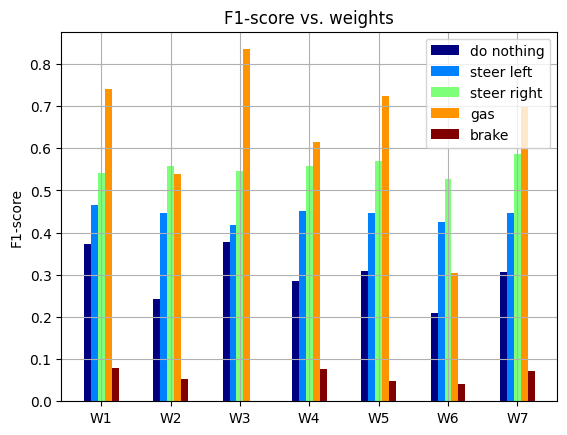
\includegraphics[width=0.4\textwidth]{figures/images/weights_f1_m0.png}
        \label{fig:weights_f1_m0}
    }
    \subfloat[Model 1.]{
        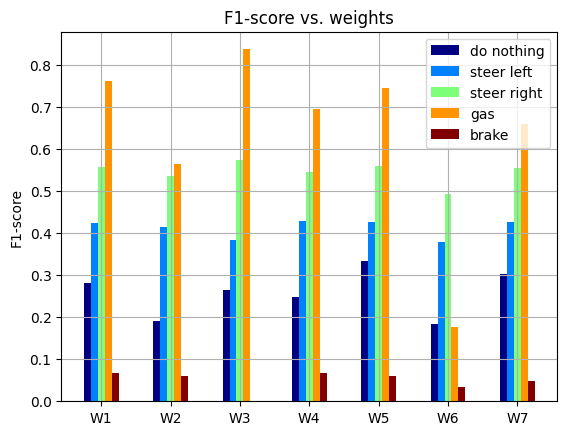
\includegraphics[width=0.4\textwidth]{figures/images/weights_f1_m1.png}
        \label{fig:weights_f1_m1}
    }
    \caption{Effect of different class weights on the class-wise f1-score.}
    \label{fig:weights_f1}
\end{figure}